\documentclass[12pt,onecolumn]{article}
\usepackage[utf8]{inputenc} % UTF8 input encoding
\usepackage[T2A]{fontenc}   % T2A font encoding for Cyrillic script
\usepackage[russian]{babel} % Russian language support
\usepackage{listings}
\usepackage{tikz}
\usepackage{float}
\usepackage{mathtools}
\everymath{\displaystyle}
\usepackage{hyperref}
\usepackage[table,xcdraw]{xcolor}
\usepackage{geometry}
\usepackage{verbatim}
\usepackage{pdfpages}
\usepackage{graphicx}
\newcommand{\nparagraph}[1]{\paragraph{#1}\mbox{}\\}
\geometry{
  a4paper,
  top=20mm, 
  right=20mm, 
  bottom=20mm, 
  left=25mm
}
\lstdefinestyle{verilog}{ 
  basicstyle=\small\ttfamily,
  commentstyle=\color{cyan},
  stringstyle=\color{magenta}\ttfamily,
  keywordstyle=\color{blue},
  numbers=left,
  numberstyle=\scriptsize,
  numbersep=5pt,
  frame=single,
  breaklines=true,
  breakatwhitespace=true,
  showstringspaces=false,
  tabsize=4,
  inputencoding=utf8,
  extendedchars=true
}

\begin{document}
\setcounter{tocdepth}{4}
\begin{center}
  Федеральное государственное автономное образовательное учреждение высшего образования "Национальный Исследовательский Университет ИТМО"\\
  Мегафакультет Компьютерных Технологий и Управления\\
  Факультет Программной Инженерии и Компьютерной Техники \\
  
\includegraphics[scale=0.3]{image/itmo.jpg} % нужно закинуть картинку логтипа в папку с отчетом
\end{center}
\vspace{1cm}


\begin{center}
  \large \textbf{Вариант №133214}\\
  \textbf{Лабораторная работа 3}\\
  по дисциплине\\
  \textbf{Тестирование программного обеспечения}
\end{center}

\vspace{2cm}

\begin{flushright}
  Выполнил Студент  группы P33102\\
  \textbf{Лапин Алексей Александрович}\\
  Преподаватель: \\
  \textbf{Харитонова Анастасия Евгеньевна}\\
\end{flushright}

\vspace{9cm}
\begin{center}
  г. Санкт-Петербург\\
  2024г.
\end{center}
\pagestyle{empty}
\newpage
\section*{Текст задания:}
Сформировать варианты использования, разработать на их основе тестовое покрытие покрытие и провести функциональное тестирование интерфейса сайта (в соответствии с вариантом).

\begin{center}
  \fbox{
    \begin{minipage}{\textwidth}
      \textbf{Вариант №133214:}

      Ucoz.ru. SaaS платформа, включающая в себя хостинг и систему управления сайтом. - http://www.ucoz.ru/
    \end{minipage}
  }
\end{center}

\textbf{Требования к выполнению работы:}
\begin{enumerate}
  \item Тестовое покрытие должно быть сформировано на основании набора прецедентов использования сайта.
  \item Тестирование должно осуществляться автоматически - с помощью системы автоматизированного тестирования Selenium.
  \item Шаблоны тестов должны формироваться при помощи Selenium IDE и исполняться при помощи Selenium RC в браузерах Firefox и Chrome.
  \item Предполагается, что тестируемый сайт использует динамическую генерацию элементов на странице, т.е. выбор элемента в DOM должен осуществляться не на основании его ID, а с помощью XPath.
\end{enumerate}
\textbf{Требования к содержанию отчёта:}
\begin{enumerate}
  \item Текст задания.
  \item UseCase-диаграмму с прецедентами использования тестируемого сайта.
  \item CheckList тестового покрытия.
  \item Описание набора тестовых сценариев.
  \item Результаты тестирования.
  \item Выводы.
\end{enumerate}

\section*{UseCase-диаграмма с прецедентами использования тестируемого сайта}

\begin{figure}[H]
  \centering
  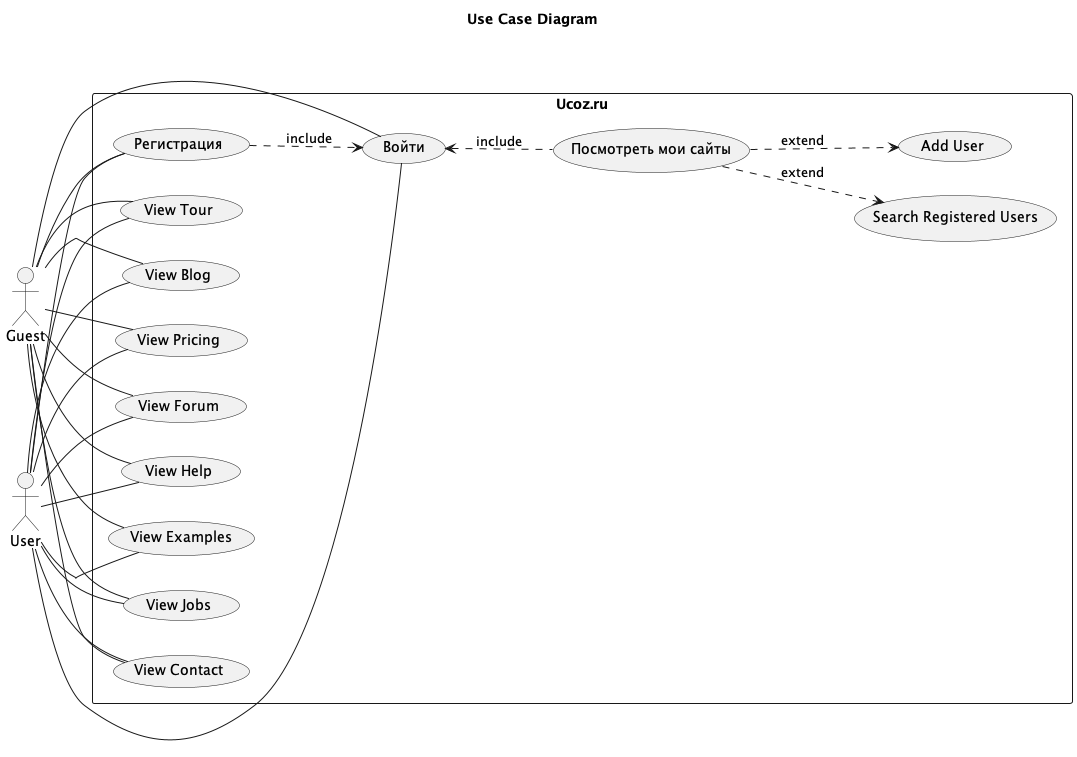
\includegraphics[width=\textwidth]{image/usecase.png}
  \caption{Use Case Diagram}
  \label{fig:usecase}
\end{figure}
\section*{CheckList тестового покрытия}
\begin{table}[H]
  \centering
  \resizebox{\columnwidth}{!}{%
    \begin{tabular}{|l|
        >{\columncolor[HTML]{32CB00}}l |
        >{\columncolor[HTML]{32CB00}}l |}
      \hline
      \cellcolor[HTML]{EFEFEF}{\color[HTML]{34CDF9} \textbf{Ucoz.ru}} & \cellcolor[HTML]{EFEFEF}\textbf{Google Chrome} & \cellcolor[HTML]{EFEFEF}\textbf{Mozilla Firefox} \\ \hline
      GuestRegistration                                               & PASSED                                         & PASSED                                           \\ \hline
      GuestAuthorisation                                              & PASSED                                         & PASSED                                           \\ \hline
      UserAuthorisation                                               & PASSED                                         & PASSED                                           \\ \hline
      UserRegistration                                                & PASSED                                         & PASSED                                           \\ \hline
      ViewBlog                                                        & PASSED                                         & PASSED                                           \\ \hline
      ViewForum                                                       & PASSED                                         & PASSED                                           \\ \hline
      ViewExamples                                                    & PASSED                                         & PASSED                                           \\ \hline
      ViewTour                                                        & PASSED                                         & PASSED                                           \\ \hline
      ViewPricing                                                     & PASSED                                         & PASSED                                           \\ \hline
      ViewJobs                                                        & PASSED                                         & PASSED                                           \\ \hline
      ViewHelp                                                        & PASSED                                         & PASSED                                           \\ \hline
      ViewContact                                                     & PASSED                                         & PASSED                                           \\ \hline
      ViewMySites                                                     & PASSED                                         & PASSED                                           \\ \hline
      ViewSitePanel                                                   & PASSED                                         & PASSED                                           \\ \hline
      SearchRegisteredUsers                                           & PASSED                                         & PASSED                                           \\ \hline
      AddUser                                                         & PASSED                                         & PASSED                                           \\ \hline
    \end{tabular}%
  }
\end{table}

\section*{Исходный код}
Можно просмотреть в моём GitHub: \href{https://github.com/AaLexUser/Software-testing}{https://github.com/AaLexUser/Software-testing}
\section*{Выводы по работе.}
В ходе выполнения данной лабораторной работы я изучил процесс тестирования веб-приложений с использованием Selenium. Научился создавать тестовое покрытие на основе прецедентов использования сайта, а также создавать и исполнять тесты в браузерах Firefox и Chrome. Также я научился работать с динамической генерацией элементов на странице, используя XPath.
\section*{Описание набора тестовых сценариев.}
\end{document}